\documentclass{article}

\usepackage[final,main]{styles/neurips_2025}

\usepackage[utf8]{inputenc}
\usepackage[T5]{fontenc}
\usepackage[vietnamese]{babel}
\usepackage{hyperref}
\usepackage{url}
\usepackage{booktabs}
\usepackage{amsfonts}
\usepackage{nicefrac}
\usepackage{microtype}
\usepackage{xcolor}
\usepackage{graphicx}
\usepackage{subcaption}
\usepackage{amsmath}
\usepackage{multirow}
\usepackage{textcomp}
\usepackage{ulem}
\usepackage{caption}
\usepackage{float}

\hypersetup{
    colorlinks=true,
    urlcolor=blue,
    linkcolor=blue,
}
\title{Dự Đoán Chi Phí Bảo Hiểm Y Tế Bằng Học Máy: \\ Từ Tiền Xử Lý Dữ Liệu Đến Tối Ưu Hóa Mô Hình}

\author{%
  Trần Trinh Nhân \\
  24280088 \\
  Trường Đại Học Khoa học Tự nhiên \\
  \url{https://github.com/TranTrinhNhan1/Medical-Insurance} \\
}

\begin{document}

\maketitle
\begin{abstract}
Dự án này thực hiện xây dựng một quy trình Machine Learning hoàn chỉnh để dự đoán chi phí bảo hiểm y tế dựa trên thông tin cá nhân. Báo cáo này trình bày chi tiết từ bước EDA, tiền xử lý, cho đến việc áp dụng các thuật toán Regression khác nhau. Kết quả thực nghiệm chỉ ra rằng các mô hình Tree-based và Gradient Boosting hoạt động hiệu quả nhất trong việc xử lý các mối quan hệ phi tuyến phức tạp. Đồng thời, nghiên cứu cũng làm sáng tỏ tầm quan trọng của việc Log Transform biến mục tiêu đối với hiệu suất của các mô hình distance-based.
\end{abstract}


\section{Introduction}

Chi phí chăm sóc sức khỏe ngày càng trở thành một gánh nặng tài chính đáng kể đối với nhiều cá nhân và gia đình. Trong bối cảnh đó, các công ty bảo hiểm y tế cần xây dựng được hệ thống tính phí bảo hiểm một cách công bằng và chính xác dựa trên hồ sơ sức khỏe và nhân khẩu học của khách hàng.

Mục tiêu của dự án là áp dụng các thuật toán Regression để dự đoán chi phí bảo hiểm y tế cá nhân (\texttt{charges}). Bằng cách xây dựng mô hình dự báo hiệu quả, chúng ta có thể:
\begin{itemize}
    \item Đánh giá mức độ tác động của các yếu tố như độ tuổi, giới tính, BMI và tình trạng hút thuốc lên chi phí y tế.
    \item Hỗ trợ các công ty bảo hiểm định giá gói cước cá nhân hóa, tối ưu hóa rủi ro và minh bạch tài chính cho khách hàng.
\end{itemize}

Dự án tuân thủ một chu trình vòng lặp Data Science tiêu chuẩn, đi từ bước tìm hiểu dữ liệu gốc, phân tích trực quan, xử lý nhiễu, cho đến việc huấn luyện đa dạng các mô hình từ cơ bản (Linear Regression, Decision Tree) đến nâng cao (Random Forest, SVR, Gradient Boosting).

\section{Dataset Description}
Dataset được sử dụng là \textbf{Medical Insurance Cost} được thu thập với tổng cộng 1338 samples và 7 features. Chi tiết các thuộc tính bao gồm:
\begin{itemize}
    \item \textbf{age}: Độ tuổi của người tham gia bảo hiểm (kiểu số nguyên).
    \item \textbf{sex}: Giới tính của người tham gia (nam/nữ).
    \item \textbf{bmi}: Body Mass Index (số thực), một trong những thước đo cơ bản để đánh giá thể trạng thừa cân.
    \item \textbf{children}: Số lượng trẻ em/người phụ thuộc được gói bảo hiểm chi trả.
    \item \textbf{smoker}: Tình trạng hút thuốc (yes/no).
    \item \textbf{region}: Khu vực sinh sống tại Mỹ (northeast, northwest, southeast, southwest).
    \item \textbf{charges} (Target variable $y$): Chi phí y tế cá nhân do bảo hiểm chi trả (kiểu số thực, đơn vị USD).
\end{itemize}

\section{Exploratory Data Analysis (EDA)}

Quá trình EDA không chỉ dừng lại ở việc quan sát thống kê mô tả, mà còn nhằm mục đích tìm ra các cấu trúc ngầm ẩn, định hướng cho việc lựa chọn mô hình và các kỹ thuật Feature Engineering về sau. Dưới đây là các phân tích chuyên sâu được bóc tách từ tập dữ liệu:

\paragraph{1. Phân phối của biến mục tiêu (\texttt{charges}) và Vấn đề Lệch chuẩn:} 
Hình \ref{fig:dist} cho thấy chi phí y tế có phân phối cực kỳ right-skewed. Hầu hết các quan sát tập trung ở vùng chi phí thấp (quanh mức 5,000 - 10,000 USD), dẫn đến việc mean bị kéo lệch đáng kể so với median. 
Đặc biệt, sự xuất hiện của vùng long tail (những bệnh nhân có chi phí y tế vượt ngưỡng 40,000 USD) tiềm ẩn nguy cơ gây ra hiện tượng Heteroscedasticity khi huấn luyện các mô hình tuyến tính. \textit{Insight} này là cơ sở vững chắc để đề xuất phương pháp Log Transform ở giai đoạn tối ưu hóa, nhằm đưa phân phối biến mục tiêu về dạng tiệm cận chuẩn, giúp các mô hình tính toán khoảng cách hội tụ tốt hơn.

\begin{figure}[H]
    \centering
    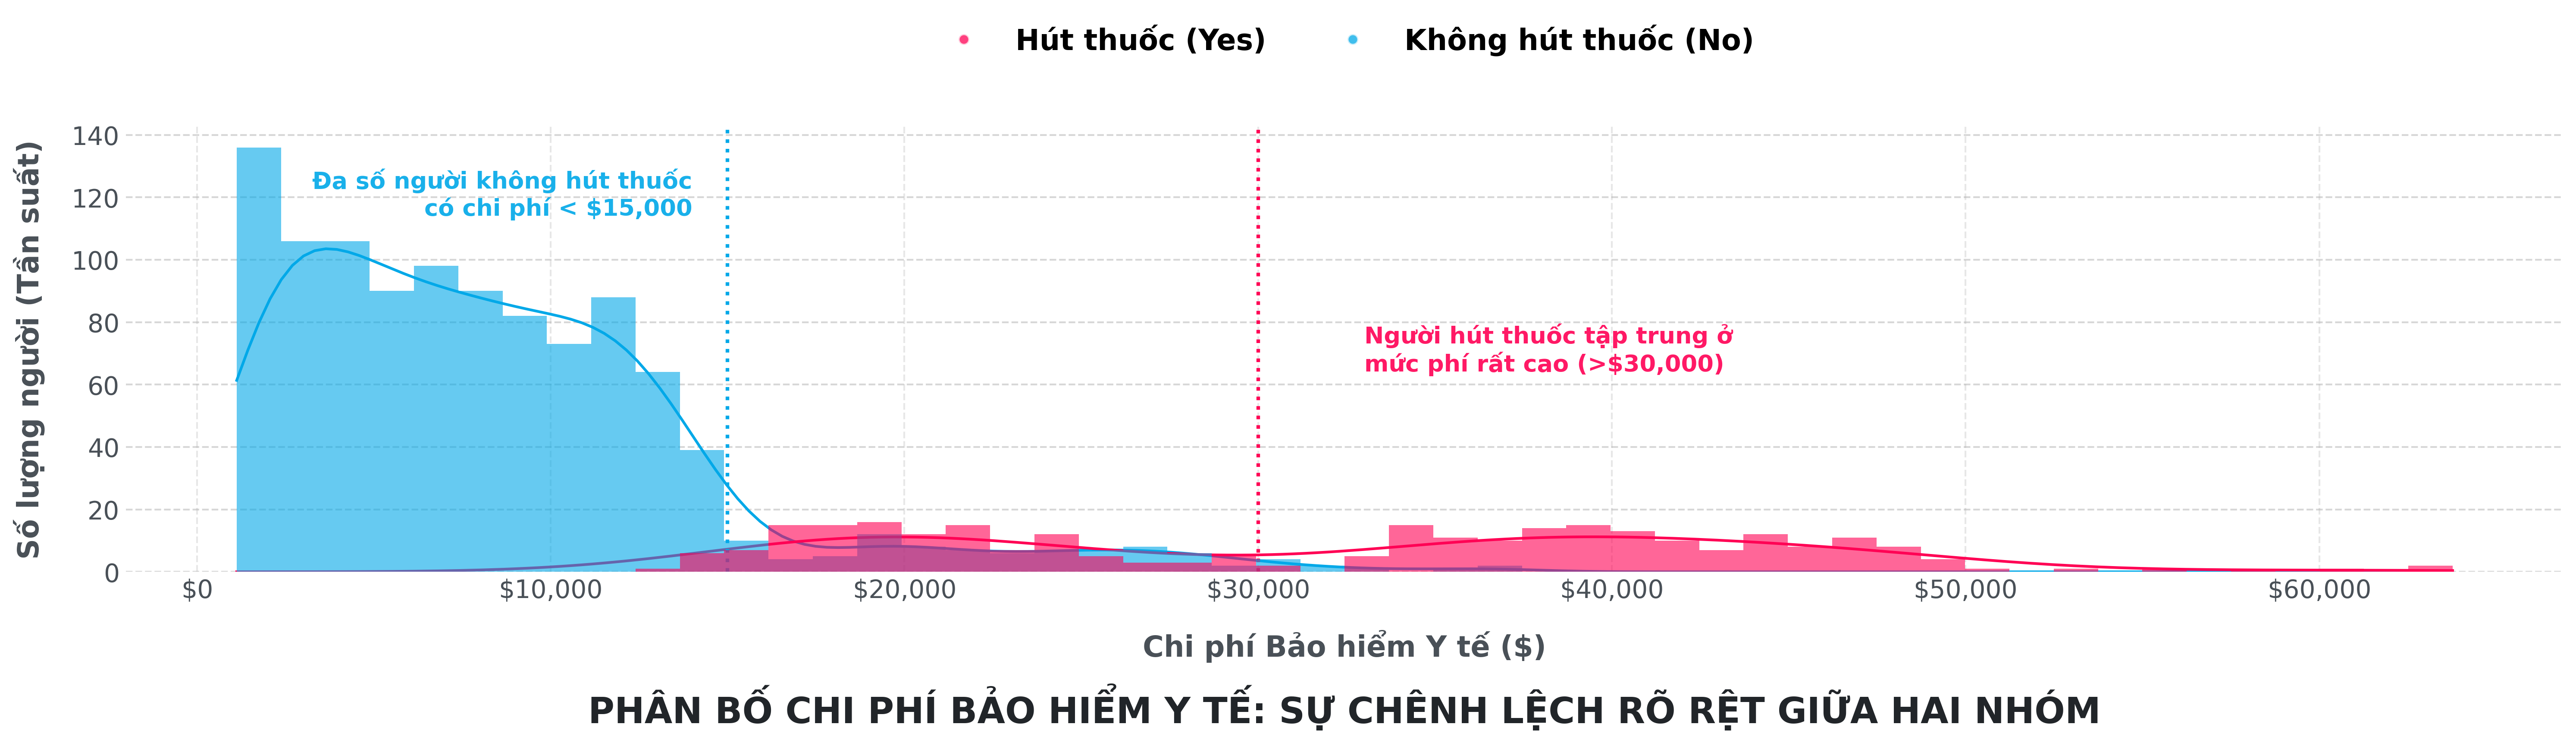
\includegraphics[width=1\linewidth]{images/Medical_Insurance_Dist.png}
    \caption{Phân phối chi phí bảo hiểm y tế (\texttt{charges}). Đuôi dài vắt sang phải cho thấy sự tồn tại của nhóm chi phí ngoại lai rất cao.}
    \label{fig:dist}
\end{figure}

\paragraph{2. Tác động thống kê của thói quen hút thuốc:} 
Biểu đồ Boxplot (Hình \ref{fig:box}) chỉ ra \texttt{smoker} là yếu tố phân loại có discriminative power lớn nhất. Ranh giới IQR giữa hai nhóm gần như không có sự giao thoa. Trung vị chi phí y tế của người hút thuốc rơi vào khoảng trên 30,000 USD, cao gấp nhiều lần nhóm không hút thuốc. Sự tách biệt tuyệt đối này ngụ ý rằng các mô hình Tree-based (như Random Forest hay LightGBM) gần như chắc chắn sẽ ưu tiên chọn biến \texttt{smoker} làm root node trong quá trình phân nhánh không gian đặc trưng.

\begin{figure}[H]
    \centering
    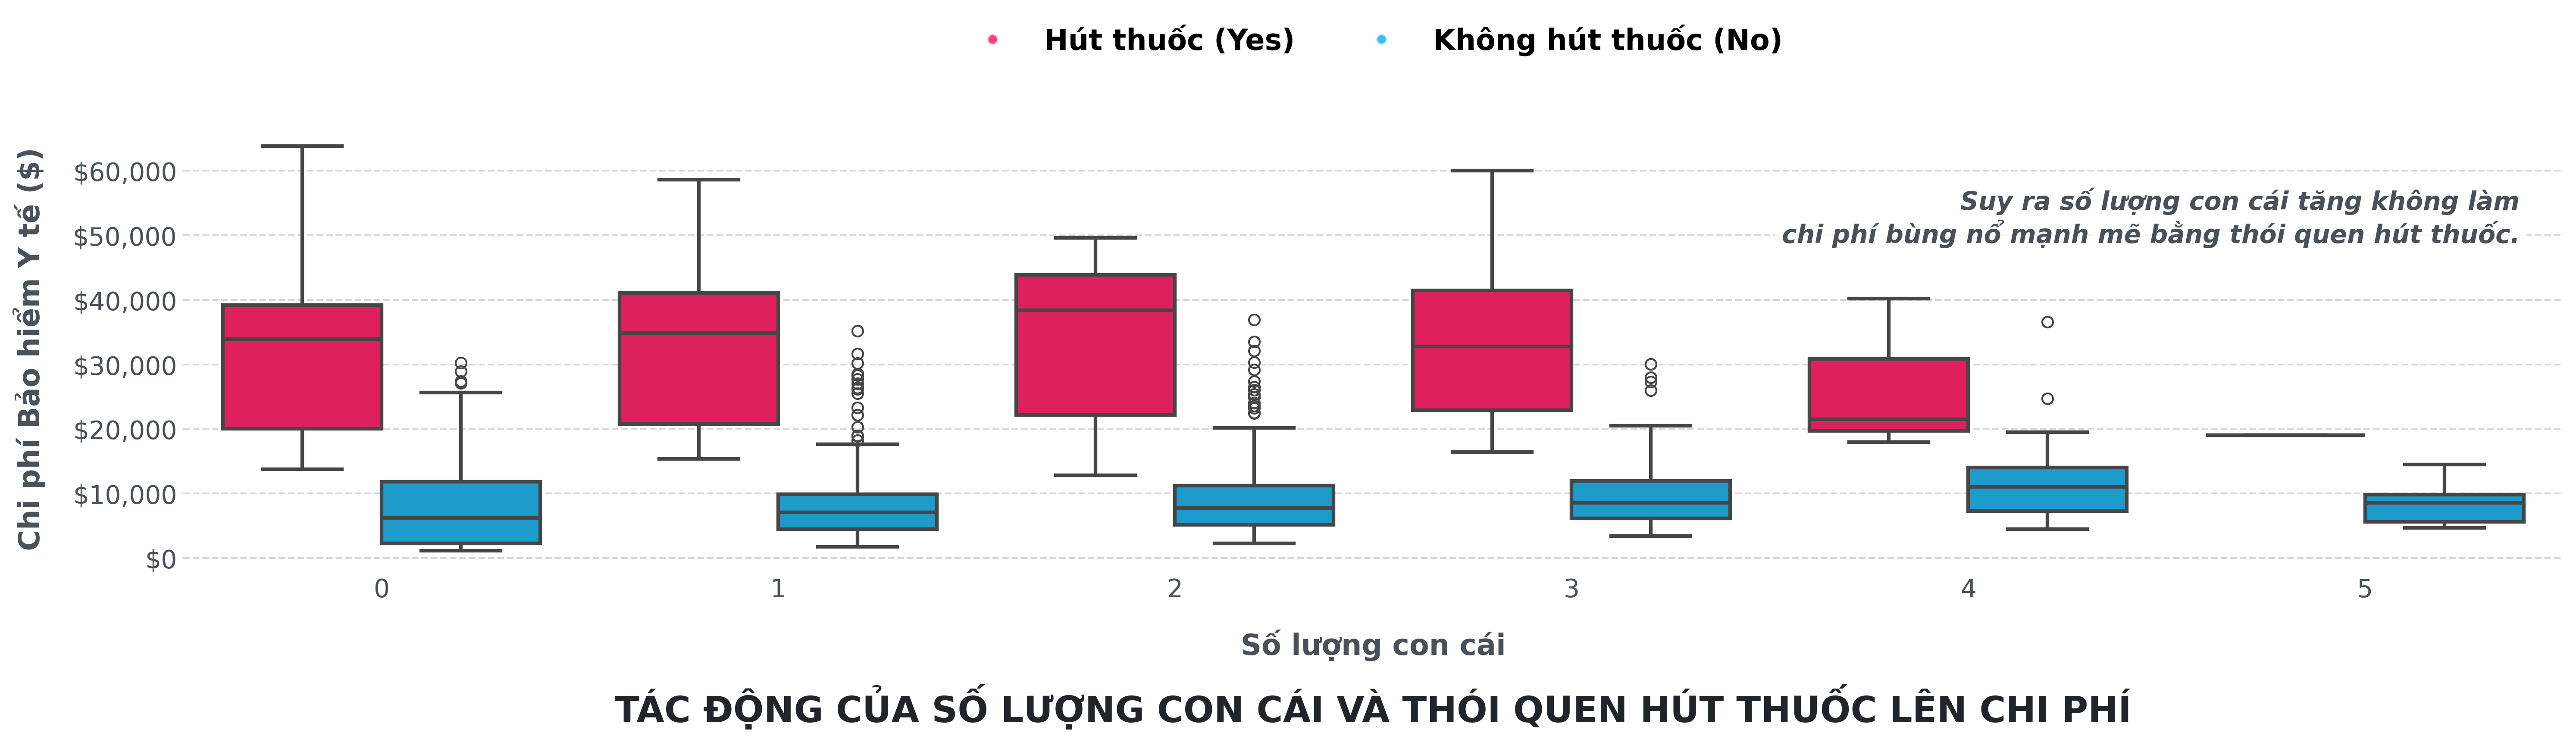
\includegraphics[width=1\linewidth]{images/Medical_Insurance_Box.png}
    \caption{Sự khác biệt về chi phí y tế theo tình trạng hút thuốc thông qua biểu đồ Boxplot.}
    \label{fig:box}
\end{figure}

\paragraph{3. Mối liên hệ phi tuyến giữa BMI, Hút thuốc và Chi phí y tế:}
Biểu đồ phân tán (Hình \ref{fig:scatter_bmi}) biểu diễn một tương tác đa biến cực kỳ thú vị. Nếu chỉ xét riêng \texttt{bmi}, độ tương quan dương với \texttt{charges} là khá yếu. Tuy nhiên, khi lồng ghép thêm yếu tố hút thuốc, dữ liệu bị chẻ làm hai cụm rõ rệt. Đáng chú ý nhất, nhóm khách hàng có BMI > 30 (ngưỡng béo phì) kèm theo thói quen hút thuốc tạo thành một cụm chi phí y tế đột biến. Sự cross-feature interaction mang tính phi tuyến này là nguyên nhân cốt lõi khiến các mô hình tuyến tính truyền thống (Linear Regression) thường thất bại, đồng thời khẳng định sự cần thiết của các mô hình có khả năng học được quy luật phi tuyến phức tạp.

\begin{figure}[H]
    \centering
    
\includegraphics[width=1\linewidth]{images/Medical_Insurance_Scatter.png}
    \caption{Tương quan giữa BMI và chi phí y tế. Cụm điểm tăng vọt phía trên cho thấy hiệu ứng cộng hưởng cực kỳ lớn giữa béo phì và hút thuốc.}
    \label{fig:scatter_bmi}
\end{figure}

\paragraph{4. Tương tác đa biến: Sự hình thành của các dải dữ liệu song song:} 
Khi quan sát chi phí y tế biến thiên theo độ tuổi (Hình \ref{fig:scatter_age}), dữ liệu hội tụ thành 3 dải đường chéo song song. Dải thấp nhất đại diện cho quy luật tự nhiên: chi phí y tế tăng nhẹ và đều đặn theo tuổi tác đối với nhóm người khỏe mạnh (không hút thuốc). Ngược lại, dải cao nhất bị chi phối hoàn toàn bởi nhóm hút thuốc kết hợp với các rủi ro sức khỏe khác. Phân tích này cũng cho thấy yếu tố giới tính (\texttt{sex}) có độ phân tán đồng đều ở cả 3 dải, hàm ý rằng giới tính có thể đóng góp Feature Importance rất thấp trong mô hình cuối cùng.

\begin{figure}[H]
    \centering
    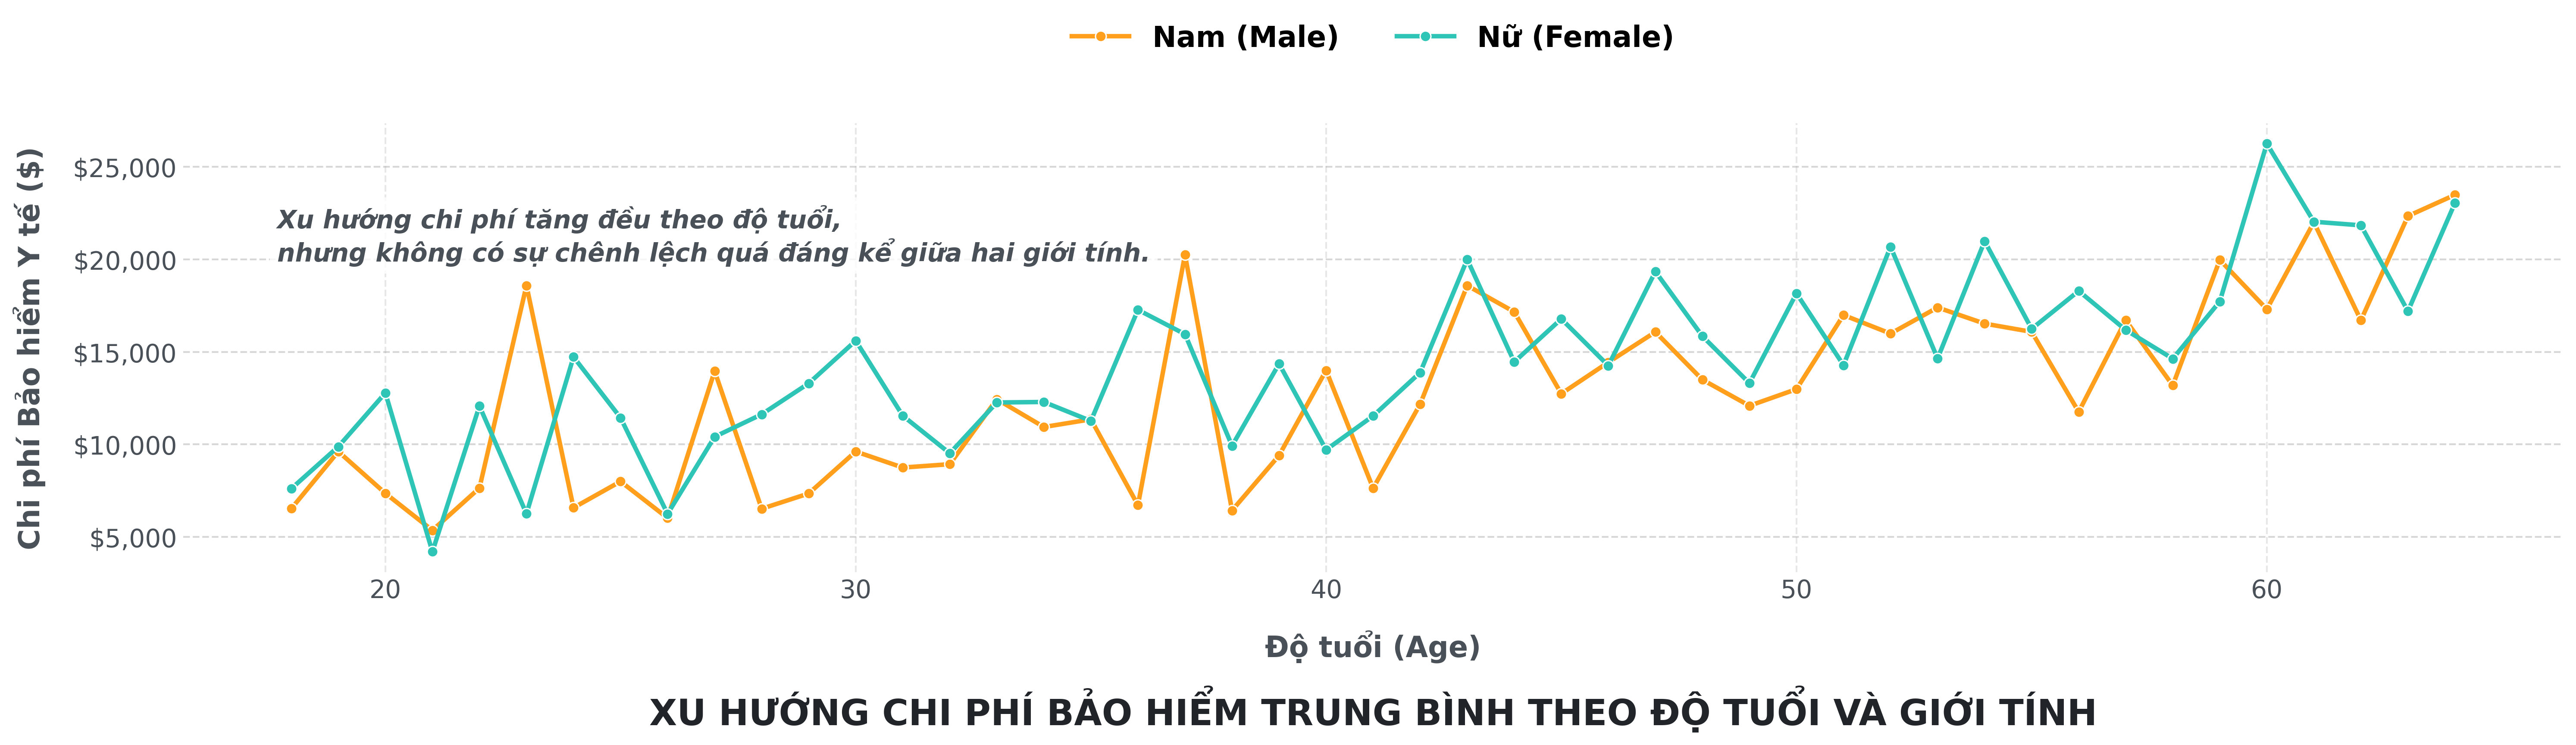
\includegraphics[width=1\linewidth]{images/Medical_Insurance_Age_Sex.png}
    
    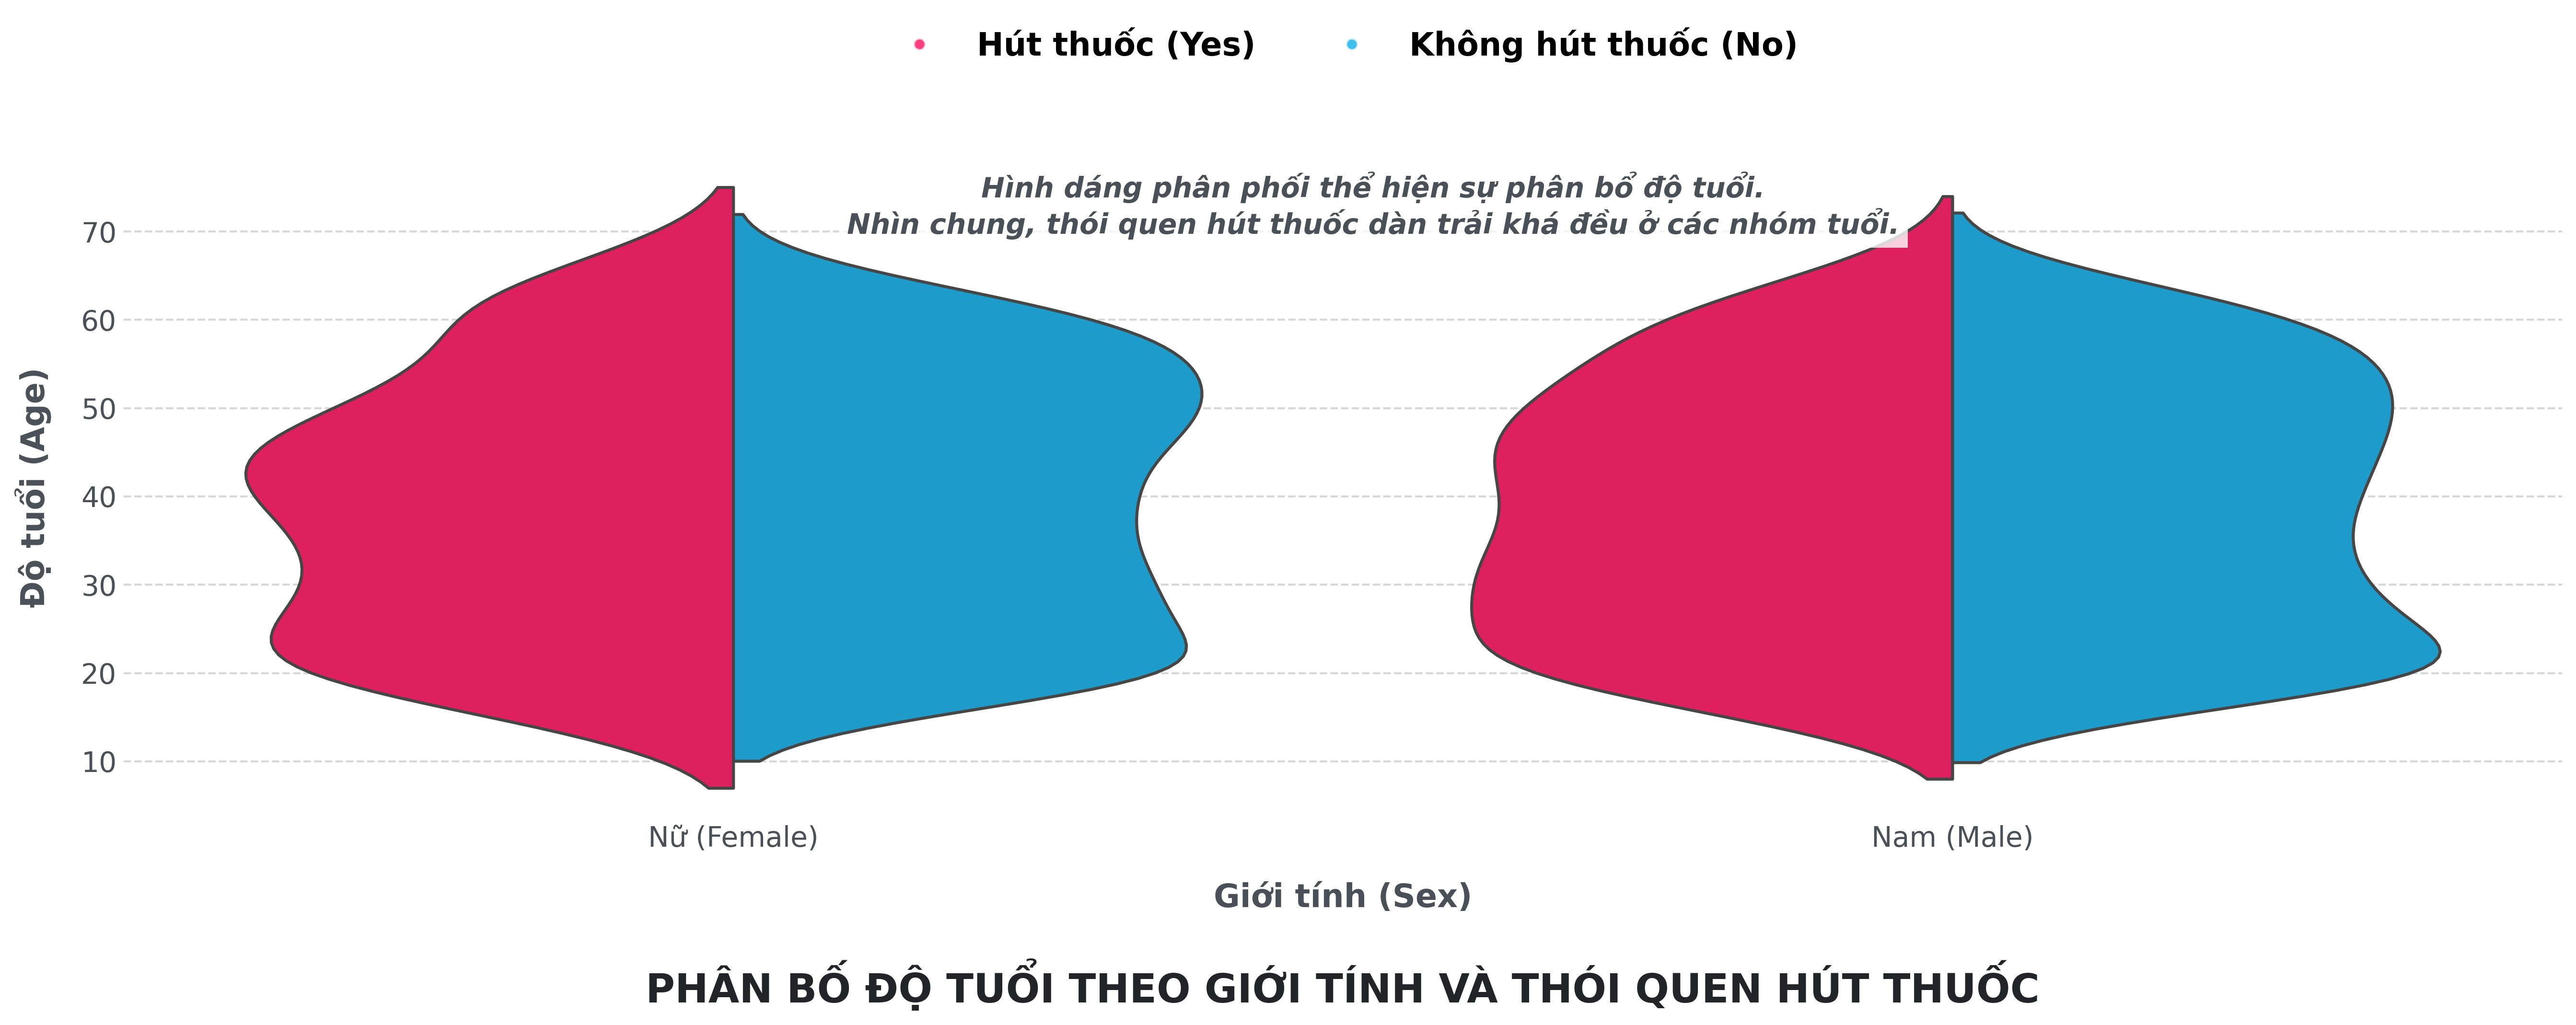
\includegraphics[width=1\linewidth]{images/Medical_Insurance_Age_Sex_Smoker.png}
    \caption{Ba dải dữ liệu song song phân tách theo độ tuổi và tình trạng hút thuốc. Giới tính không tạo ra sự phân biệt rõ ràng.}
    \label{fig:scatter_age}
\end{figure}

\paragraph{5. Tính toàn vẹn và Phân bổ của Categorical Features:}
Biểu đồ Bar chart (Hình \ref{fig:bar}) cung cấp cái nhìn vĩ mô về thiết kế thu thập dữ liệu. Các biến phân loại như khu vực sinh sống (4 vùng tại Mỹ) và giới tính đều có sự phân bổ quan sát xấp xỉ nhau. Sự vắng bóng của hiện tượng Class Imbalance bảo đảm rằng ta không cần phải can thiệp bằng các kỹ thuật resampling (như SMOTE) hay Class Weights. Các mô hình hoàn toàn có thể tự tin học trên dữ liệu nguyên bản mà không lo bị bias về một phân khúc khách hàng đa số nào.

\begin{figure}[H]
    \centering
    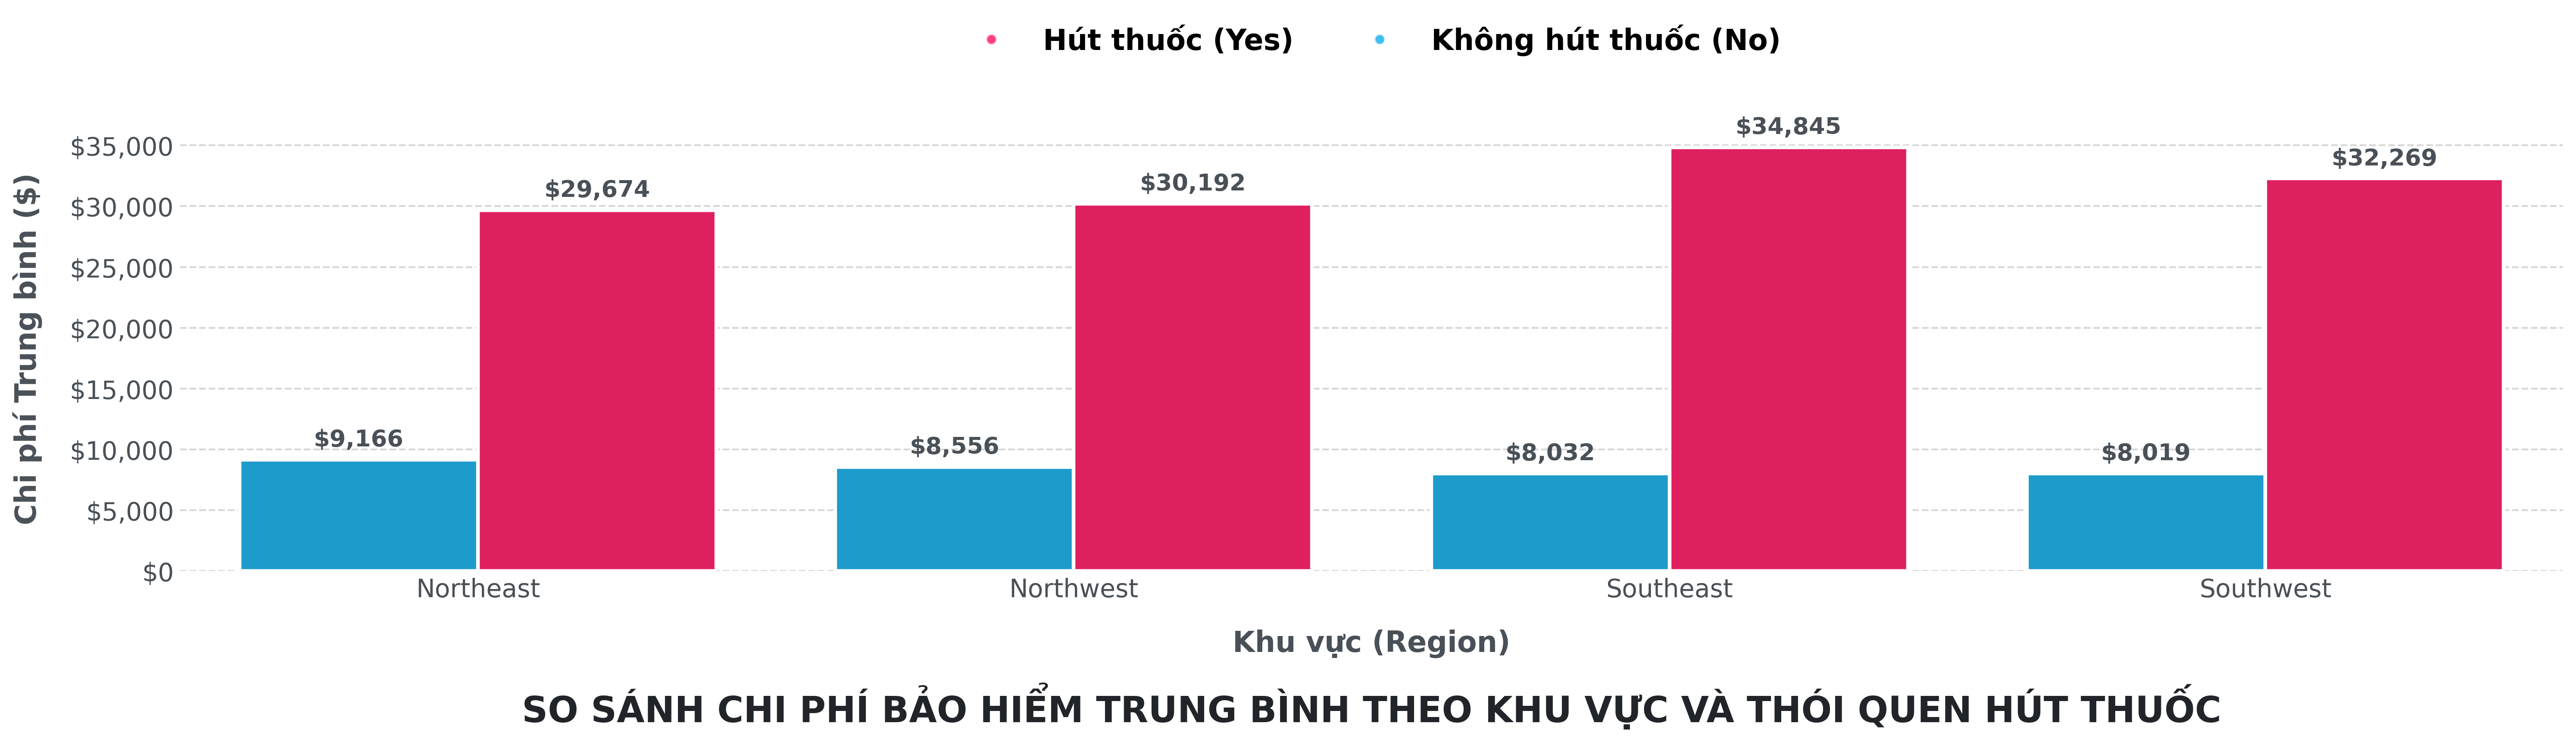
\includegraphics[width=1\linewidth]{images/Medical_Insurance_Bar.png}
    \caption{Phân bố tần suất đồng đều của các biến phân loại, xác nhận không có nhiễu loạn từ hiện tượng Class Imbalance.}
    \label{fig:bar}
\end{figure}

\section{Data Preprocessing}

Quá trình Data Preprocessing đóng vai trò quyết định nhằm loại bỏ nhiễu và định dạng lại dữ liệu sao cho phù hợp với đầu vào của các thuật toán Machine Learning. Để tránh hiện tượng Data Leakage — nơi mô hình học được thông tin từ Test Set — quy trình được thiết kế cẩn trọng qua các bước sau:

\begin{enumerate}
    \item \textbf{Data Cleaning}: Quét và xóa 1 dòng dữ liệu trùng lặp. Đặc biệt, phân tích IQR trên cột \texttt{bmi} phát hiện và loại bỏ 9 outliers, giúp các mô hình giảm nhiễu trước khi huấn luyện.
    \item \textbf{Feature Engineering}: Dựa trên insight từ EDA, một đặc trưng mới \texttt{is\_smoker\_obese} được tạo ra. Khách hàng vừa hút thuốc vừa có \texttt{bmi} > 30 sẽ nhận giá trị 1, ngược lại là 0. Điều này giúp các mô hình Linear Regression nắm bắt ngay được tương tác chéo cực độ này mà không cần cơ chế phân nhánh phức tạp.
    \item \textbf{Train/Test Split}: Tập dữ liệu được phân chia ngẫu nhiên thành hai phần theo tỷ lệ 80\% (Train) và 20\% (Test) với \texttt{random\_state=42} để đảm bảo tính reproducibility.
    \item \textbf{Categorical Encoding linh hoạt}: Các categorical features (\texttt{sex}, \texttt{smoker}, \texttt{region}) được biến đổi bằng \texttt{OneHotEncoder}. Cấu hình được tinh chỉnh động tùy theo mô hình:
    \begin{itemize}
        \item Mô hình tuyến tính (Linear/SVR): Sử dụng \texttt{drop='first'} để loại bỏ một phân lớp, tránh hiện tượng multicollinearity chết người.
        \item Mô hình dựa trên cây (Decision Tree/Random Forest): Sử dụng \texttt{drop=None} để giữ lại tất cả các cột, giúp thuật toán phân tách đối xứng tự nhiên hơn.
    \end{itemize}
    \item \textbf{Feature Scaling}: Các numerical features (\texttt{age}, \texttt{bmi}, \texttt{children}, \texttt{is\_smoker\_obese}) được scale về mean = 0 và variance = 1 thông qua \texttt{StandardScaler}. Scaler này chỉ được \texttt{fit} chặt chẽ trên tập Train.
\end{enumerate}

Toàn bộ các quy trình biến đổi tính năng trên được đóng gói bằng đối tượng \texttt{ColumnTransformer} và \texttt{Pipeline} của \texttt{scikit-learn}, đảm bảo toàn bộ quy trình đi từ Raw Data đến Model Prediction là một flow không bị ngắt quãng.

\section{Models}

Để tìm ra phương pháp dự báo giá trị \texttt{charges} tối ưu, năm thuật toán cơ bản đã được lựa chọn huấn luyện:
\begin{itemize}
    \item \textbf{Linear Regression}: Mô hình Linear Regression cơ bản, làm baseline đo lường.
    \item \textbf{Decision Tree Regressor}: Mô hình Decision Tree, dễ hiểu trực quan nhưng dễ gặp overfitting.
    \item \textbf{Random Forest Regressor}: Thuật toán Ensemble mạnh mẽ, xây dựng đa dạng hóa thông qua tập hợp nhiều Decision Tree.
    \item \textbf{K-Nearest Neighbors (KNN)}: Thuật toán distance-based.
    \item \textbf{Support Vector Regressor (SVR)}: Thuật toán cố gắng tìm ra một hyperplane bao trọn tối đa các điểm dữ liệu bên trong biên độ sai số $\epsilon$.
\end{itemize}

\subsection{Hyperparameter Tuning}
Mặc định, các mô hình khởi tạo với tham số tiêu chuẩn có thể không tận dụng được tối đa tiềm năng dữ liệu. Do đó, kỹ thuật \textbf{GridSearchCV} kết hợp với \textbf{K-Fold Cross-Validation (K=5)} được áp dụng trên tập Train để tự động rà soát parameter grid:
\begin{itemize}
    \item \textbf{Random Forest}: Tìm kiếm giá trị tối ưu cho \texttt{max\_depth} và \texttt{n\_estimators}.
    \item \textbf{Decision Tree}: Tinh chỉnh \texttt{max\_depth} và \texttt{min\_samples\_split}.
    \item \textbf{KNN}: Lựa chọn \texttt{n\_neighbors} và \texttt{weights} (uniform vs distance).
    \item \textbf{SVR}: Khảo sát biên độ rộng với \texttt{C} (từ 0.1 đến 1000) và \texttt{gamma} nhằm tìm ra mặt phẳng tốt nhất cho biến mục tiêu có phương sai lớn.
\end{itemize}
Bước này không chỉ cải thiện độ chính xác mà điểm \textbf{CV Mean R2 Score} thu được còn đóng vai trò tham chiếu tuyệt vời để kiểm tra mức độ Overfitting khi đối chiếu với Test Score.

\section{Results}

Các mô hình được đánh giá thông qua tập Test và Cross-validation (K=5) trên tập Train. Sự kết hợp giữa CV Score và Test Score cho phép chúng ta có cái nhìn toàn diện về độ ổn định của mô hình. Kết quả chi tiết được trình bày tại Bảng \ref{tab:results}.

\begin{table}[H]
  \caption{Bảng So Sánh Hiệu Suất Các Mô Hình (Đã qua Hyperparameter Tuning \& Outlier Removal)}
  \label{tab:results}
  \centering
  \begin{tabular}{lrrrrr}
    \toprule
    Mô hình & CV Mean R2 & MAE & MSE & RMSE & Test R2 \\
    \midrule
    Linear Regression & \textbf{0.8607} & 2479.03 & 20,506,677 & 4528.43 & 0.8525 \\
    Decision Tree & 0.8404 & 3124.28 & 30,342,130 & 5508.37 & 0.7817 \\
    Random Forest & 0.8561 & 2546.18 & 20,048,804 & 4477.59 & \textbf{0.8558} \\
    K-Nearest Neighbors & 0.8234 & 3023.20 & 27,092,844 & 5205.08 & 0.8051 \\
    Support Vector Regressor & 0.8284 & \textbf{1889.45} & 23,060,624 & 4802.15 & 0.8341 \\
    \bottomrule
  \end{tabular}
\end{table}

\section{Compare Models}

\subsection{Linear Regression \& Feature Engineering Synergy}
Trong số các thuật toán, \textbf{Linear Regression} đã có màn trình diễn xuất sắc và bất ngờ nhất với điểm CV Mean R2 cao nhất (\textbf{0.8607}) và Test R2 = 0.8525. Thành công này đến trực tiếp từ bước Feature Engineering khi bổ sung biến \texttt{is\_smoker\_obese}. Khác với trước đây khi Linear Regression chỉ mô tả được xu hướng tuyến tính phẳng và thất bại trước tương tác chéo, việc cung cấp sẵn cross-feature interaction này đã giúp mô hình tuyến tính vượt qua cả các thuật toán phức tạp.

\subsection{Random Forest Regressor}
Dù không còn dẫn đầu tuyệt đối về mọi mặt, \textbf{Random Forest} vẫn thể hiện sự ổn định tuyệt vời với Test R2 cao nhất (\textbf{0.8558}). Sức mạnh này đến từ:
\begin{itemize}
    \item \textbf{Tính chất Ensemble:} Bằng cách xây dựng hàng ngàn Decision Tree khác nhau dựa trên việc bootstrap \& feature bagging, Random Forest giảm thiểu đáng kể vấn đề High Variance thường thấy ở Decision Tree đơn lẻ.
    \item \textbf{Nắm bắt quan hệ phi tuyến:} Thuật toán phân mảnh không gian theo dạng bậc thang, cho phép mô hình dễ dàng tự học được các cross-feature interactions cực kỳ phức tạp ngay cả khi không có Feature Engineering.
\end{itemize}

\subsection{Support Vector Regressor (SVR) Performance Analysis}
Trước khi thực hiện tối ưu, kết quả kiểm thử cho thấy SVR đạt hiệu suất cực kỳ thấp (R2 Score âm). Tuy nhiên, sau khi áp dụng \textbf{GridSearchCV} và tìm ra bộ tham số tối ưu (\texttt{C=1000.0}, \texttt{gamma=0.1}), SVR đã đạt được \textbf{MAE thấp nhất (1889.45)}. 
Sự lột xác này chứng minh tầm quan trọng của Hyperparameter Tuning:
\begin{itemize}
    \item Việc tăng \texttt{C=1000.0} đã ép hyperplane hội tụ chính xác hơn trên các biên dữ liệu, cho phép SVR tối thiểu hóa sai số tuyệt đối (MAE) vô cùng hiệu quả.
\end{itemize}

\subsection{Overfitting Evaluation}
Nhờ việc bổ sung Cross-validation (K=5), chúng ta có thể đánh giá mức độ Overfitting một cách rõ ràng. Sự chênh lệch giữa \textbf{CV Mean R2} và \textbf{Test R2} ở hầu hết các mô hình là rất nhỏ (dưới 0.02). Ví dụ, Random Forest có CV R2 là 0.8561 và Test R2 là 0.8558. Điều này khẳng định quy trình Train/Test Split ban đầu kết hợp với Data Cleaning đã đại diện tốt cho toàn bộ không gian dữ liệu, và mô hình có khả năng generalization xuất sắc.

\section{Conclusion \& Bonus Pipeline}

\subsection{Model Optimization Experiment}
Để tiếp tục nâng cao hiệu suất, một \textbf{Bonus Pipeline} cải tiến đã được thiết kế và thực thi với hai hướng tiếp cận:
\begin{enumerate}
    \item \textbf{Cân bằng phân phối biến mục tiêu:} Áp dụng Log Transform (\texttt{np.log1p}) cho $y$ trong quá trình huấn luyện và khôi phục giá trị thực thông qua \texttt{np.expm1} ở bước dự đoán. Cơ chế này được tự động hóa thông qua \texttt{TransformedTargetRegressor}.
    \item \textbf{Áp dụng thuật toán Gradient Boosting:} Đưa vào các kiến trúc Ensemble tiên tiến hơn là XGBoost và LightGBM nhằm tăng cường tốc độ và độ chính xác so với thuật toán Random Forest cơ bản.
\end{enumerate}

\begin{table}[H]
  \caption{Kết Quả Mô Hình Sau Khi Áp Dụng Bonus Pipeline}
  \label{tab:bonus_results}
  \centering
  \begin{tabular}{lrrrr}
    \toprule
    Mô hình & MAE & MSE & RMSE & R2 Score \\
    \midrule
    Log Transformed Linear Regression & 3755.92 & 51,797,278 & 7197.03 & 0.7181 \\
    Log Transformed SVR & 2518.39 & 29,148,483 & 5398.93 & 0.8414 \\
    XGBoost & 2663.22 & 25,971,562 & 5096.23 & 0.8587 \\
    \textbf{LightGBM} & \textbf{2344.66} & \textbf{20,436,077} & \textbf{4520.63} & \textbf{0.8888} \\
    \bottomrule
  \end{tabular}
\end{table}

\subsection{Conclusion}
Dựa trên Bonus Pipeline, mô hình \textbf{LightGBM} cho thấy hiệu năng vượt trội, đạt giá trị MAE thấp nhất (2344.66) và R2 Score cao nhất (\textbf{0.8888}). Đáng chú ý là Log Transform lại làm giảm hiệu suất của Linear Regression do đặc trưng \texttt{is\_smoker\_obese} có quan hệ tuyến tính trực tiếp với giá trị gốc của \texttt{charges} hơn là giá trị Log.

Nghiên cứu đã hoàn thành mục tiêu xây dựng và dự báo chi phí y tế. Qua đó, kết quả thực nghiệm khẳng định tầm quan trọng của Data Preprocessing, Feature Engineering và Hyperparameter Tuning. Mô hình LightGBM được đề xuất làm phương pháp tối ưu nhất cho bài toán này.

\subsection{Challenges \& Future Work}
\textbf{Khó khăn gặp phải:}
\begin{itemize}
    \item Dữ liệu có đặc thù lệch phải mạnh, gây khó khăn cho các mô hình tuyến tính nếu không có Feature Engineering phù hợp.
    \item Việc tối ưu GridSearchCV tốn khá nhiều tài nguyên tính toán đối với cấu trúc Ensemble phức tạp như XGBoost hay LightGBM.
\end{itemize}

\textbf{Hướng cải thiện trong tương lai:}
\begin{itemize}
    \item Thu thập thêm dữ liệu từ các nguồn đa dạng hơn để tránh tình trạng phân phối tập trung vào một số cụm giá trị đặc thù.
    \item Áp dụng các kỹ thuật AutoML tiên tiến như Optuna để tìm kiếm không gian siêu tham số nhanh và tối ưu hơn so với thuật toán Grid Search truyền thống.
\end{itemize}


\end{document}
